\documentclass[a4paper]{article}

\usepackage{fullpage} % Package to use full page
\usepackage{parskip} % Package to tweak paragraph skipping
\usepackage{tikz} % Package for drawing
\usepackage{amsmath}
\usepackage{hyperref}

\title{Circus Specification}
\author{Ashley J. Robinson}
\date{\today}

\begin{document}

\maketitle

\section{Introduction}

   \subsection{Acronyms} 
      \begin{table}[h]
         \centering
         \caption{Acronyms}
         \label{tab_acronyms}
         \begin{tabular}{|l|l|}
            \hline
            \textbf{Acronyms}    &  \textbf{Description}                         \\ \hline  
            CMD                  &  Command                                      \\ \hline
            GUI                  &  Graphical User Interface                     \\ \hline
            ID                   &  Identity                                     \\ \hline
            IR                   &  Infra-Red                                    \\ \hline
            LED                  &  Light Emitting Diode                         \\ \hline
            OOK                  &  On-Off Keying                                \\ \hline
            PC                   &  Personal Computer                            \\ \hline
            PW                   &  Parity Word                                  \\ \hline
            UART                 &  Universal Asynchronous Receiver-Transmitter  \\ \hline  
            USB                  &  Universal Serial Bus                         \\ \hline
         \end{tabular}
\end{table}  


\section{Agent}

   \subsection{ID}
      \begin{itemize}
         \item Agents have hardware pin straps to configure IDs
         \item Agents have a valid ID range of 0x01 to 0xFE inclusive
         \item Agent ID = pin strap value + 1
      \end{itemize}
  
   \subsection{CMD}
      \begin{itemize}
         \item The list off \textbf{CMDs} is held in Table~\ref{tab_cmds}. 
      \end{itemize}
 
      \begin{table}[h]
         \centering
         \caption{Valid agent \textbf{CMDs}}
         \label{tab_cmds}
         \begin{tabular}{|l|l|l|l|l|l|}
               \hline
               \textbf{CMD}   &  \textbf{Control}     &  \textbf{Green LED}   &  \textbf{Red LED}  &  \textbf{Left Motor}  &  \textbf{Right Motor} \\ \hline  
               0x00           &                       &                       &                    &                       &  Off                  \\ \hline   
               0x01           &                       &                       &                    &                       &  Forward slow         \\ \hline   
               0x02           &                       &                       &                    &                       &  Forward              \\ \hline   
               0x03           &                       &                       &                    &                       &  Forward fast         \\ \hline   
               0x04           &                       &                       &                    &                       &  Reverse slow         \\ \hline   
               0x05           &                       &                       &                    &                       &  Reverse              \\ \hline   
               0x06           &                       &                       &                    &                       &  Reverse fast         \\ \hline   
               ...            &                       &                       &                    &                       &                       \\ \hline   
               0x10           &                       &                       &                    &  Off                  &                       \\ \hline   
               0x11           &                       &                       &                    &  Forward slow         &                       \\ \hline   
               0x12           &                       &                       &                    &  Forward              &                       \\ \hline   
               0x13           &                       &                       &                    &  Forward fast         &                       \\ \hline   
               0x14           &                       &                       &                    &  Reverse slow         &                       \\ \hline   
               0x15           &                       &                       &                    &  Reverse              &                       \\ \hline   
               0x16           &                       &                       &                    &  Reverse fast         &                       \\ \hline   
               ...            &                       &                       &                    &                       &                       \\ \hline   
               0x20           &                       &                       &  Force off         &                       &                       \\ \hline   
               0x21           &                       &                       &  Force on          &                       &                       \\ \hline   
               0x22           &                       &                       &  Low battery       &                       &                       \\ \hline   
               0x23           &                       &                       &  Full battery      &                       &                       \\ \hline   
               0x24           &                       &                       &  Blink on rx       &                       &                       \\ \hline   
               0x25           &                       &                       &  Blink on tx       &                       &                       \\ \hline   
               ...            &                       &                       &                    &                       &                       \\ \hline   
               0x30           &                       &  Force off            &                    &                       &                       \\ \hline   
               0x31           &                       &  Force on             &                    &                       &                       \\ \hline   
               0x32           &                       &  Low battery          &                    &                       &                       \\ \hline   
               0x33           &                       &  Full battery         &                    &                       &                       \\ \hline   
               0x34           &                       &  Blink on rx          &                    &                       &                       \\ \hline   
               0x35           &                       &  Blink on tx          &                    &                       &                       \\ \hline   
               ...            &                       &                       &                    &                       &                       \\ \hline   
               0x80           &  Shut down            &                       &                    &                       &                       \\ \hline   

         
         \end{tabular}
      \end{table}


\section{Communications}
 
\begin{itemize}
   \item The communication scheme overview is shown in Figure~\ref{fig_communications}. 
   \item Communication is achieved using and \textbf{IR} link.
   \item The carrier for the link is 38KHz.
   \item The carrier will be modulated with a \textbf{UART} using \textbf{OOK}.
   \item The \textbf{UART} baud rate will be 9600.
   \item The \textbf{UART} will carry 8 bits of data.
   \item The \textbf{UART} will 1 start/stop bit.
   \item The \textbf{UART} will not contain a parity bit.
   \item The \textbf{UART} will not use flow control.
\end{itemize}



\begin{figure}[h]
   \centering
   \label{fig_communications}
   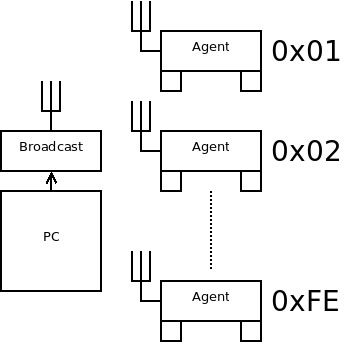
\includegraphics[width=6cm,keepaspectratio]{communications/communications.png} 
   \caption{Communication overview.}
\end{figure}

   \subsection{Broadcast}
      \begin{itemize}
         \item The IR receiver will be connected to UART transmitter of a microcontroller. 
         \item The \textbf{UART} signal will gate the carrier.
         \item The broadcaster will be connected to a \textbf{PC}.
         \item The \textbf{PC} will us a \textbf{GUI} application to control the broadcaster.
         \item The microcontroller used to control the broadcast will communicate
               with the \textbf{PC} using low speed \textbf{USB}.
      \end{itemize}

 
   
   \subsection{Receiver}
      \begin{itemize}
         \item The IR receiver will be connected to UART receiver of the microcontroller. 
         \item The receiver is initially in the \textbf{OFF} state. 
         \item The recover polls every 200ms for a carrier.
         \item The receiver must successfully find a carrier in two adjacent polls to switch the 
               receiver in to the \textbf{ON} state.
         \item Once in the \textbf{ON} state the receiver will constantly monitor the presence 
               of a carrier and return to the `\textbf{OFF} state when the carrier is lost. 
               This is 
      \end{itemize}

      \begin{figure}[h]
         \centering
         \label{fig_communications_time}
         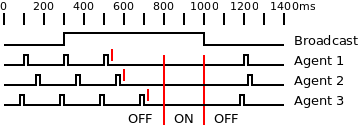
\includegraphics[width=10cm,keepaspectratio]{communications/communications_time.png} 
         \caption{Communication initiate timeout.}
      \end{figure}



\begin{itemize}
   \item    The agent receiver state machine is shown in Figure~\ref{fig_communications_sm}.
   \item    0xFF is invalid in both the \textbf{ID} and \textbf{CMD} states and will 
            push the state back to idle \textbf{ID} state. This can be used to reset the state machine
            as flushing with 0xFF will have no action.
   \item    Unmatching IDs will be stalled to allow \textbf{CMD} and \textbf{PW} to pass which may clash with valid \textbf{IDs}. 
   \item    Valid agents are shown in Table~\ref{tab_ids}.
   \item    Upon leaving the \textbf{ID} state an action must be reached before 50ms.
            An example of a completed and timed out transaction is shown in Figure~\ref{fig_communications_wave}.
   \item    The 
\end{itemize}

\begin{figure}[h]
   \centering
   \label{fig_communications_sm}
   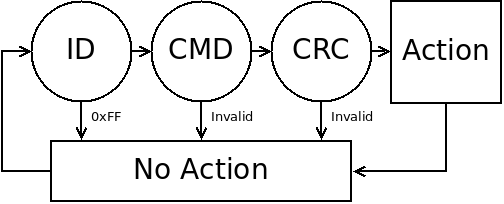
\includegraphics[width=8cm,keepaspectratio]{communications/communications_sm.png} 
   \caption{Communication state machine.}
\end{figure}

\begin{figure}[h]
   \centering
   \label{fig_communications_wave}
   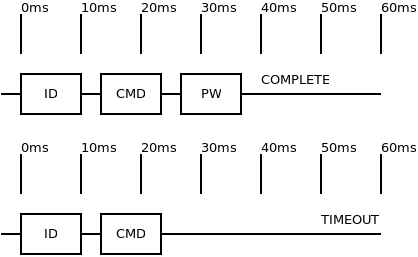
\includegraphics[width=8cm,keepaspectratio]{communications/communications_wave.png} 
   \caption{Communication message timeout.}
\end{figure}



\begin{table}[h]
   \centering
   \caption{Valid agent IDs.}
   \label{tab_ids}
   \begin{tabular}{|l|l|l|l|l|l|}
        \hline
        \textbf{ID}  &  \textbf{Description} \\ \hline  
         0x00        &  Issue the following command to all agents.\\ \hline  
         0x01..0xFE  &  Issue the following command to all agents with matching IDs.\\ \hline  
         0xFF        &  Resets the agent receiver state machine. \\ \hline  
   \end{tabular}
\end{table}



\section{GUI}
   \begin{itemize}
      \item The \textbf{GUI} will contain a tick box for every valid agent \textbf{ID}. 
      \item The \textbf{GUI} will contain a broadcast tick box which will disable all \textbf{ID}
            tick boxes.
      \item The \textbf{GUI} will contain a button to force a reset. 
      \item The arrow keys will be mapped to the directional control of the agents.
      \item The G key will be mapped to cycle through the green \textbf{LED}.
      \item The R key will be mapped to cycle thorugh the red \textbf{LED}
      \item The \textbf{GUI} will contain a text box streaming raw \textbf{CMDs} being set to the agents.
   \end{itemize}



\end{document}

